\section{Source reconstruction, validation, and measured performance}
\label{sec:experiments}

The experiments answer three separate questions: whether the finite
algorithms agree with independent exhaustive oracles; whether the native
source compiler supplies the claimed graph--matrix inputs; and how the
exact strategies compare on the same saved instances. None of these
experiments proves a worst-case parameter bound for knot diagrams.

\subsection{Finite oracle and certificate validation}

The ordered suite contains 16 test methods, 5,129 forest-oracle
comparisons, and 800 independently brute-forced cloned-Rado comparisons.
The output-assignment suite contains nine methods and 6,024 forest-oracle
comparisons. Both finish with zero failures, errors, or skips. These are
algorithm--instance comparisons: the suites intentionally overlap, so
their sum is not a count of distinct mathematical inputs.

The exhaustive part ranges over all $3^{3\cdot2}=729$ capped
three-row, two-column matrices on four different cap geometries, for
2,916 comparisons per included sweep. Independent oracles enumerate top
trees and, in the designated tests, all legal positive raw pivots. Random
tests cover unit triples, larger exceptional supports, nonunit entries,
loops, and unavailable rows. Focused controls cover shared prerequisite
witnesses, initially free graph edges, unsupported cyclic dependencies,
complete-negative coverage, and the distinguished block's undemanded
semantics.

The raw-parity tests deliberately use counts three and two. They verify
that saturation cannot authorize a rank shortcut and that changing an
uncapped integer invalidates a source-bound certificate even when the
unit-peeling predicate is unchanged. Additional checks exercise a
16,384-bit multiplicity and a comparably large disconnected vertex
namespace without expanding that namespace.

\subsection{A fresh native reconstruction}

The maintained marked-parallelity corpus contains 106 cases. We add three
interior-loop cuts, five stellar-subdivision cases, and three nested
interior-subdivision cases from the inspected incoming geometric fixtures.
This gives 117 triangulation/normal-vector cases, each producing a source
matrix and a full finite-boundary matrix: 234 correlated finite questions.

For each case the experiment reconstructs the complementary handle core,
fixes and records the lower forest, counts the original attaching
occurrences, and independently derives cap endpoints from the source
triangulation representatives. The endpoint map is compared with the
incoming cap compiler. Annular crossings and finite boundary relations are
also reconstructed independently and compared with the earlier boundary
adapter after saturation. The saved record includes actual face pairings,
normal coordinates, row maps, raw profiles, source hashes, and exact
reference decisions.

Every one of the 234 full raw inputs satisfies the cap-parity condition.
All maintained full-boundary columns have raw total at most three, and
every active exceptional column is a unit triple. Fifteen maintained
full-boundary cases contain sixteen single-owner columns with raw count
three. Their owners must be matroid loops because these particular raw
inputs satisfy parity, so saturation does not alter cap parity for these
single-owner columns. They demonstrate raw-source fidelity and digest
binding; the mixed-column controls above demonstrate parity sensitivity
in general. Only the uncapped
reconstruction is distributed as the authoritative input bank.

The independent all-top-tree oracle completes on every maintained source
and full-boundary matrix. It also completes on every supplementary case
except the largest stellar input, where its explicit 250,000-subset cap
is recorded. The older exact stopping-set search completes on all 117
cases, including that largest input, and provides a checked reference
answer there. A capped exhaustive oracle is never reported as complete.

\begin{center}
\begin{tabular}{@{}llrrr@{}}
\toprule
Strategy & Maintained matrix & Success & No forest & Inconclusive \\
\midrule
Earlier two-row solver & Source & 81 & 0 & 25 \\
Earlier two-row solver & Full boundary & 67 & 2 & 37 \\
Earlier stopping search & Source & 100 & 6 & 0 \\
Earlier stopping search & Full boundary & 92 & 14 & 0 \\
Either new exact strategy & Source & 100 & 6 & 0 \\
Either new exact strategy & Full boundary & 92 & 14 & 0 \\
\bottomrule
\end{tabular}
\end{center}

Thus the new methods resolve the nonlinear cases declined by the old
polynomial special-case solver. They reproduce the coverage already
obtained by the previous general exact criterion. This experiment does
not add new whole-knot recognitions or increase the maintained full-cut
success count beyond 92.

Free closure substantially changes the parameter distribution. In the
maintained source matrices the residual $k$ distribution is
$0:98,\ 1:7,\ 2:1$. In the full boundary matrices it is
$0:95,\ 1:9,\ 3:1,\ 9:1$. The large-parameter negative is rejected by
a short immutable obstruction before exceptional enumeration. These
observations justify the preprocessing, but are not evidence that every
future hierarchy has logarithmically many nonlinear columns.

\begin{figure}[tb]
\centering
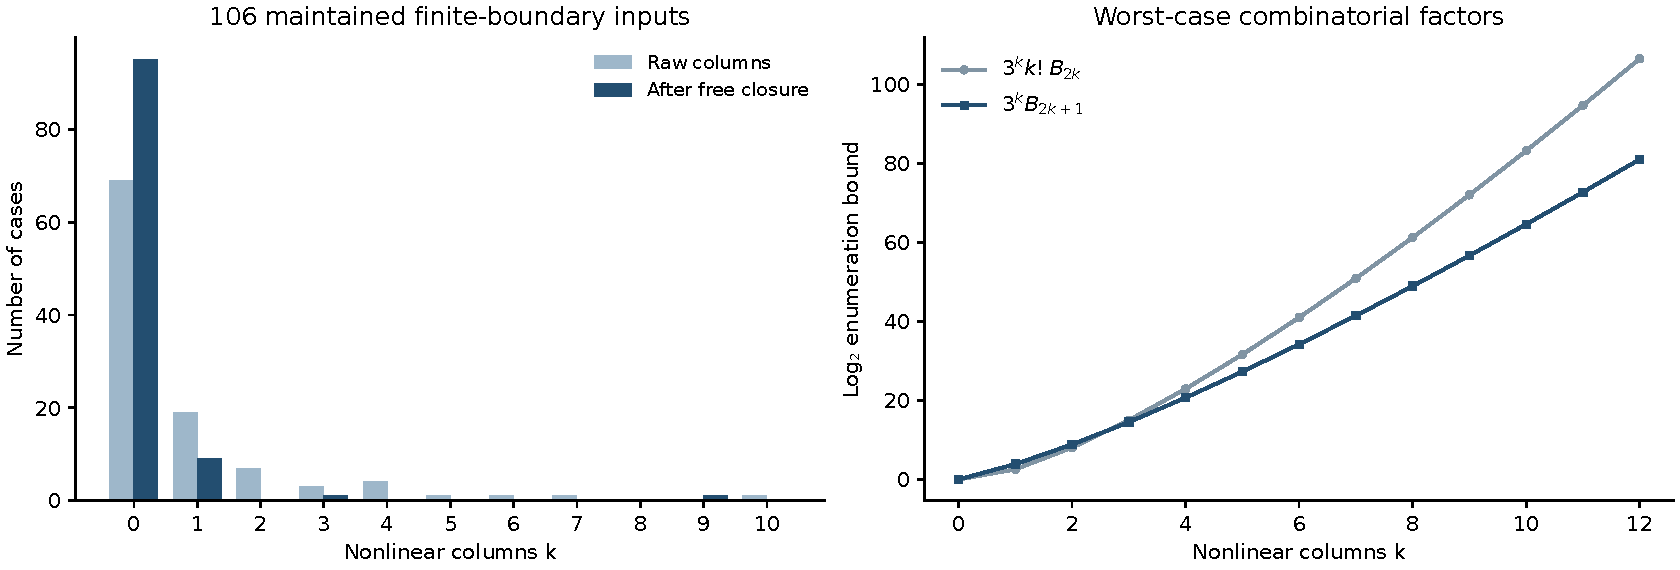
\includegraphics[width=\linewidth]{figures/parameters_and_bounds.pdf}
\caption{Left: measured raw and residual nonlinear parameters on the 106
maintained full-boundary inputs. Right: exact general enumeration factors
before data-dependent rank and closure pruning. The right panel depicts
combinatorial upper bounds, not measured running times.}
\label{fig:parameters}
\end{figure}

\subsection{Supplementary native stress cases and resource ceilings}

At a one-million structural-work allowance, the ordered strategy completes
228 of 234 questions: source $107/7/3$ and full boundary $99/15/3$, where
the entries denote success, no forest, and inconclusive. The output-only
strategy completes 232: source $109/7/1$ and full boundary $101/15/1$.
Every completed result is independently replayed and agrees with the
earlier exact reference. The only remaining output-only cap is the largest
stellar case, in both matrix variants.

The deterministic structural counters expose genuine improvements between
the two new strategies. On \texttt{stellar\_torus/3}, with residual $k=6$,
the count falls from 426,223 to 742. The output-only method completes
\texttt{stellar\_torus/4}, $k=9$, in 12,682 units, and
\texttt{nested\_interior\_torus/3}, $k=9$, in 397; the ordered strategy
reaches its cap on both. A unit of this instrumented work is not a machine
instruction or a portable elapsed-time unit. Counts from the older
implementation use different instrumentation and are not directly equated.

\subsection{Paired timings and ablations}

The paired benchmark uses all 117 native full-boundary matrices and 256
seeded relabelings described below, for 373 finite inputs. Each is run
seven times with a seeded random ordering of the six methods inside each
repetition. This yields 15,666 timed calls. Every complete timed answer
is independently checked outside the timer; there are 13,475 such
replays. Inconclusive results remain in the raw table.

The environment is CPython 3.12.14 on Linux. Geometry construction,
parameter reporting, and certificate replay are outside the timed region;
input parsing and search are inside it. The two new algorithms use the
same one-million work cap and are each run with rank pruning enabled and
disabled. The earlier stopping search uses its own 50,000-node cap;
these different counters do not represent equal computational budgets.
The machine-readable result retains every raw repetition, status, counter,
input hash, and code hash. Microsecond-scale timings characterize this run,
not a machine-independent performance promise.

\begin{center}
\begin{tabular}{@{}lrrrr@{}}
\toprule
Method & Success & No forest & Inconclusive & Median ($\mu$s) \\
\midrule
Earlier two-row solver & 67 & 2 & 37 & 42.80 \\
Earlier stopping search & 92 & 14 & 0 & 43.64 \\
Ordered events & 92 & 14 & 0 & 79.24 \\
Output assignments & 92 & 14 & 0 & 82.86 \\
\bottomrule
\end{tabular}
\end{center}


The output-only implementation has higher overhead than the existing
stopping search on most small instances. On the maintained corpus its
median per-input time is about 83 microseconds, compared with 44 for the
incumbent. Across the entire bank, it is faster on 16 of the 372 inputs
where both methods complete. The improvement in the parameterized
worst-case guarantee is therefore not a justification for replacing the
incumbent unconditionally.

\begin{center}
\begin{tabular}{@{}lrrrr@{}}
\toprule
Input & $k$ & Ordered (ms) & Output (ms) & Incumbent (ms) \\
\midrule
Stellar 1 & 0 & 0.068 & 0.080 & 0.058 \\
Stellar 2 & 3 & 0.111 & 0.129 & 0.143 \\
Stellar 3 & 6 & 309.743 & 0.614 & 0.296 \\
Stellar 4 & 9 & capped & 7.737 & 0.441 \\
Stellar 8 & 21 & capped & capped & 2.271 \\
Nested 1 & 1 & 0.135 & 0.139 & 0.165 \\
Nested 2 & 6 & 0.164 & 0.180 & 0.346 \\
Nested 3 & 9 & capped & 0.369 & 0.607 \\
\bottomrule
\end{tabular}
\end{center}


On the $k=6$ stellar case, the ordered median is 309.743 milliseconds
and the output-only median is 0.614 milliseconds, about a 505-fold
improvement. The incumbent still completes that input in 0.296
milliseconds. On the final nested case the output-only method takes
0.369 milliseconds, versus 0.607 for the incumbent, while the ordered
prototype is capped. Both favorable and unfavorable comparisons belong
in the integration decision.

The rank ablation is consequential on the harder stellar inputs. Removing
rank pruning changes the output-only $k=6$ median from 0.614 to 4.317
milliseconds, and makes its $k=9$ stellar run hit the work cap. It has
little or negative constant-factor effect on many tiny cases. The
largest stellar instance remains a useful counterweight to favorable
benchmarks: the incumbent finishes it in 2.271 milliseconds, while the
new output-only solver is still capped.

\subsection{Relabeling one source and evaluating the bounded prefix}

The 256 relabelings permute tetrahedra and local corners of the same
five-tetrahedron solid-torus zero cut, using seed 20261012471. The complete
finite tree oracle finds a successful tree in every instance. Native BFS
top selection succeeds on 238, and the existing native maximum-weight
choice succeeds on all 256. Both new exact solvers also succeed on all
256, with independently replayed saved certificates. These are labeled
variants of one manifold, not 256 new knot types. Since maximum weight
already covers the entire bank, the bank does not demonstrate additional
coverage from the new exact search.

The optional dispatcher in Section~\ref{sec:bounded-prefix} runs the
incumbent for at most $|R|+1$ search nodes before the FPT fallback. It
completes all 490 supplied source/full-boundary and relabeled questions,
with 468 successes and 22 exact negatives. Every answer is independently
checked. In this bank the incumbent always finishes within the prefix;
its maximum instrumented count is nine visited search nodes. Explicit separate controls exercise successful and negative
fallback certificates and the sparse huge-namespace route. These results
establish dispatcher correctness on the bank, not a measured speedup for
the wrapper or a universal nine-node bound.

\subsection{What can be reproduced without the repository}

The archive includes all finite input matrices, both runtime strategies,
their independent checkers, the pinned earlier finite comparator, saved
certificates, the full paired timing table, and a single reproduction
entry point. Those finite experiments require only the Python standard
library. Figure generation additionally uses Matplotlib; article building
uses a standard \LaTeX{} installation.

Reconstructing the native source geometry again requires the pinned
maintained runtime and the two named incoming geometry packages. The
included scripts accept explicit paths to them. Their file identities
and the source input vectors are retained, so this dependency is
reviewable and is not hidden behind the previously generated matrices.
